\documentclass[10pt,oneside]{article}
\usepackage{amsmath} 
\usepackage{graphicx} 
\usepackage{subcaption} 
\usepackage{amsfonts}
\usepackage{amssymb} 


\newcommand{\tr}{\operatorname{tr}}
\newcommand{\diag}{\operatorname{diag}}
\newcommand{\adj}{\operatorname{adj}}
\newcommand{\vecm}{\operatorname{vec}}

\newcommand{\dotstar}{\operatorname{.*}}


\usepackage{pgf, tikz}
\usetikzlibrary{arrows, automata, quotes}

\usepackage{minted}

\usepackage[utf8]{inputenc}
\usepackage{upgreek}
\DeclareUnicodeCharacter{2248}{$\approx$}
\DeclareUnicodeCharacter{2218}{$\circ$}
\DeclareUnicodeCharacter{2297}{$\otimes$}
\DeclareUnicodeCharacter{2081}{$_1$}
\DeclareUnicodeCharacter{2082}{$_2$}
\DeclareUnicodeCharacter{2083}{$_3$}

% \usepackage[
%   backend=biber
% ]{biblatex}
% \addbibresource{biblio.bib}


\usepackage[
  letterpaper,
  left=1cm,
  right=1cm,
  top=1.5cm,
  bottom=1.5cm
]{geometry}


\usepackage{hyperref}

\usepackage{enumitem}

\usepackage{lastpage}
\usepackage{fancyhdr}
\fancyhf{}
\pagestyle{fancy}
\fancyhf{}
\fancyhead[L]{MIT IAP January 2025} 
\fancyhead[C]{18.063 Matrix Calculus} 
\fancyhead[R]{Profs. Edelman and Johnson} 
\fancyfoot[R]{}
% https://tex.stackexchange.com/questions/227/how-can-i-add-page-of-on-my-document
\fancyfoot[C]{\thepage\ of \pageref*{LastPage}}
%\fancyfoot[C]{ of }
\fancyfoot[L]{} 
\renewcommand{\headrulewidth}{2pt} 
\renewcommand{\footrulewidth}{2pt}

\author{} 
\title{Homework 2 Solutions}

\date{\today}


\DeclareCaptionFormat{mitedFormat}{%
    \textbf{#1#2}#3}
\DeclareCaptionStyle{minetdStyle}{skip=0cm,width=.85\textwidth,justification=centering,
  font=footnotesize,singlelinecheck=off,format=mitedFormat,labelsep=space}
\newenvironment{mintedCode}{\captionsetup{type=listing,style=minetdStyle}}{}

\usepackage{dirtytalk} 


\usepackage[parfill]{parskip}

\usepackage{csquotes} 

\begin{document}
%\input{julia_font}
%\input{julia_listings}

\maketitle
\thispagestyle{fancy} 

{\bf See also the accompanying Julia notebook for computational solutions.  }

\subsection*{Problem 1 (5 points)}

Continue reading the draft course notes (linked from \url{https://github.com/mitmath/matrixcalc/}).   Find another place that you found confusing, in a different chapter from your answer in homework~1, and write a paragraph explaining the source of your confusion and (ideally) suggesting a possible improvement.

(Any other corrections/comments are welcome, too.)

\subsubsection*{Solution:}

Student-dependent, but full marks if clearly written and explained.

\subsection*{Problem 2  (5+5+5 points)}

Consider the following system $g(x,p)=0$ of two nonlinear equations
in two variables $x\in\mathbb{R}^{2}$, parameterized by three parameters
$p\in\mathbb{R}^{3}$:
\[
g(x,p)=\left(\begin{array}{c}
p_{1}x_{1}^{2}-x_{2}\\
x_{1}x_{2}-p_{2}x_{2}+p_{3}
\end{array}\right)=\left(\begin{array}{c}
0\\
0
\end{array}\right).
\]
For $p=[1,2,1]$ this has an exact solution $x=[1,1]$.
\begin{enumerate}
\item What are the Jacobian matrices $\frac{\partial g}{\partial x}$ and
$\frac{\partial g}{\partial p}$? (That is, as defined in class, the
linear operators such that $dg=\frac{\partial g}{\partial x}dx+\frac{\partial g}{\partial p}dp$
for any change $dx$ and $dp$, to first order.)
\item In Julia (or Python etc.), implement Newton's method to solve $g(x,p)=0$
from a given starting guess~$x$. Using $p=[1,2,1]$, start your
Newton iteration at $x=[1.2,1.3]$ and show that it converges rapidly
to $x=[1,1]$ (it should converge to machine precision in $<10$ steps).
\item Now, consider the function $f(p)=\Vert x(p)\Vert$, where the ``implicit
function''\footnote{This $x(p)$ can be defined uniquely in some neighborhood of a root
like the one above, thanks to the implicit-function theorem.} $x(p)$ is a solution of $g(x,p)=0$. Given a solution $x(p)$ for
some $p$, explain how to compute $\nabla f$ (see the adjoint-method
notes from lecture~5). Implement this algorithm in Julia (etc.),
and validate it against a finite-difference approximation for $p=[1,2,1]$,
$x(p)=[1,1]$, and a random small $\delta p$ (solving for $x(p+\delta p)$
by Newton's method starting from $x(p)$).
\end{enumerate}

\subsubsection*{Solution:}

\begin{enumerate}
    \item 

     $\frac{\partial g}{\partial x}=
     \begin{pmatrix}
     2p_1x_1 & -1 \\  x_2 & x_1-p_2
     \end{pmatrix},  \ \
      \frac{\partial g}{\partial p}=
       \begin{pmatrix}
     x_1^2 &  0 & 0 \\  0 & -x_2 & 1
     \end{pmatrix}.$
    \item  See accompanying Julia notebook.

    \begin{center}
% \begin{mdframed}[backgroundcolor=backgroundcolor, rightline=false]
%     \lstinputlisting[language=Julia, style=julia, frame={}]{newtonstep.jl}
% \end{mdframed}
\end{center}


 \item  As explained in the lecture-5 slides and the course notes, $df = -f'(x) \left( \frac{\partial g}{\partial x} \right)^{-1} \frac{\partial g}{\partial p} dp = (\nabla f)^T dp$.  Here, $f = \Vert x \Vert \implies f' = \frac{x^T}{\Vert x \Vert}$ (from pset 1), so we can transpose to obtain:
 $$
 \boxed{\nabla f = -\left(\frac{\partial g}{\partial p}\right)^T \left[ \underbrace{ \left(\frac{\partial g}{\partial x} \right)^{-T} \frac{x}{\Vert x \Vert}}_v \right] }\, ,
 $$
 where the brackets indicate that we want to compute it in the order shown: first compute the ``adjoint'' solution $v$ (similar in cost to a single step of Newton's method), and then multiply it by $\left(\frac{\partial g}{\partial p}\right)^T $, all evaluated at the current $p$ and $x(p)$.

 See the accompanying Jupyter notebook to solve this problem numerically and validate it against a finite-difference solution.

Although you were \emph{not required} to do so, in this particular case, we can solve everything analytically. For $p = [1,2,1]$, we have $x = [1,1]$ and hence $\frac{\partial g}{\partial x}= \begin{pmatrix} 2 & -1 \\  1 & -1 \end{pmatrix} $, giving (using the standard formula for the inverse of a $2 \times 2$ matrix, noting that this matrix has determinant $-1$):
 $$
 \nabla f = -\frac{1}{\sqrt{2}}\underbrace{\begin{pmatrix}
     1 & 0 \\ 0 & -1 \\ 0 & 1
     \end{pmatrix}}_{\left(\frac{\partial g}{\partial p}\right)^T} \left[ \underbrace{\begin{pmatrix}
     1 & 1 \\ -1 & -2
     \end{pmatrix}}_{\left(\frac{\partial g}{\partial x} \right)^{-T}} 
     \begin{pmatrix}
     1 \\ 1
     \end{pmatrix}
      \right] = \frac{1}{\sqrt{2}} \begin{pmatrix}
     -1 & 0 \\ 0 & 1 \\ 0 & -1
     \end{pmatrix} \begin{pmatrix}
     2 \\ -3 
     \end{pmatrix} = \boxed{\frac{1}{\sqrt{2}} \begin{pmatrix}
     -2 \\ -3 \\ 3 
     \end{pmatrix} \approx \begin{pmatrix}
      -1.414214 \\
 -2.121320 \\
  2.121320
     \end{pmatrix}} \, .
 $$
\end{enumerate}


\subsection*{Problem 3 (10 points)}

In pset~1, you checked numerically that if $Aq_k = \lambda_k q_k$, where $A=A^T$ is a real-symmetric matrix and $q_k^T q_k=1$, then $\nabla \lambda_k(A) = q_k q_k^T$.   We will show a nice derivation of this in class.

% \begin{enumerate} \item 
Alternatively, you should be able to derive this by implicit differentiation: since $\lambda_k$ is a root $g=0$ of $g(\lambda,A) = \det(A - \lambda I)$, apply the determinant-gradient formula to show that $\nabla \lambda_k(A) = q_k q_k^T$.

Hint: the determinant gradient involves the adjugate matrix $\operatorname{adj}(M)$, which is normally obtained as $M^{-1} \det M$, but the latter formula doesn't work if $M$ is singular.  Instead, write the adjugate in terms of the diagonalization of $A$ and take the limit $\lambda \to \lambda_k$ in order to obtain a formula that works when the determinant is zero.

\subsubsection*{Solution:}

For our implicit function $\lambda(A)$ defined by $g(\lambda,A) = 0$, we use $dg = \frac{\partial g}{\partial A}[dA] + \frac{\partial g}{\partial \lambda} d\lambda$, which as in class we can solve for
$$
d\lambda = -\left(\frac{\partial g}{\partial \lambda}\right)^{-1} \frac{\partial g}{\partial A}[dA] = \langle \nabla_A \lambda, dA \rangle = \tr((\nabla_A \lambda)^T dA) \, ,
$$
where $\partial g/\partial \lambda$ is a scalar and the rhs is just the definition of $\nabla_A \lambda$ in terms of the Frobenius inner product.  Now, let's see if we can simplify these terms to solve for $\nabla_A \lambda$.

Recall that $d(\det M) = \tr(\adj(M) dM)$ where $\adj M$ is the adjugate matrix: it equals $M^{-1} \det M$ for non-singular $M$, and more generally is the transpose of the cofactor matrix of $M$.  Let $M(\lambda) = A - \lambda I$.  Hence, by the chain rule, we have
$$
\frac{\partial g}{\partial \lambda} = \tr(\adj(M) M'(\lambda) ) = -\tr(\adj(M)) \,
$$
since $M'(\lambda) = -I$ (similar to problem 5.2 of pset~1), and
$$
\frac{\partial g}{\partial A}[dA] = \tr(\adj(M) dA ) \, .
$$
In both cases, we need to compute $\adj M$, and we need to do so at our root $\lambda = \lambda_k$ (one of the eigenvalues of $A$).   The tricky part is that $M(\lambda_k)$ is singular (by definition of an eigenvalue), so we can't use the usual adjugate formula involving $M^{-1}$.

Instead, let's take the hint and use the diagonalizaiton $A = Q \Lambda Q^T$ of $A$, where the columns of $Q$ are the orthonormal eigenvectors $q_k$ and the diagonal elements of $\Lambda$ are the real eigenvalues $\lambda_k$ (noting that $A$ is real-symmetric so that it has such a diagonalization).   Then $M(\lambda) = A - \lambda I = Q (\Lambda - \lambda I) Q^T$ has the same eigenvectors, but eigenvalues shifted by $\lambda$.  First, let's consider the case where $\lambda$ is \emph{not} an eigenvalue, so that we can use the explicit adjugate formula:
$$
\adj M = M^{-1} \det M = Q (\Lambda - \lambda I)^{-1} Q^T \det(\Lambda - \lambda I) = Q \adj(\Lambda - \lambda I) Q^T \, ,
$$
where the adjugate of the diagonal matrix $\Lambda - \lambda I$ is easy: you just invert the diagonal entries and multiply by the determinant (the product of the diagonal entries).  When you do this, however, the diagonal entry that you are dividing by \emph{cancels} the corresponding entry from the determinant, and you are left with diagonal entries:
$$
(\Lambda - \lambda I)_{ii} = \prod_{j \ne i} (\lambda_j - \lambda) \, .
$$
\emph{Now} we can take the limit as $\lambda \to \lambda_k$ (\emph{one} of the eigenvalues), and we see that all of the diagonal terms vanish (because they contain $\lambda_k - \lambda_k$) \emph{except} for the $k$-th term, leaving us with a rank-1 matrix:
$$
\adj M(\lambda_k) = \left[ \prod_{j \ne k} (\lambda_j - \lambda_k) \right] q_k q_k^T \, .
$$
Moreover, $-\tr(\adj(M(\lambda_k))) = -\tr(\adj(\Lambda - \lambda_k I))$ simply becomes $-\prod_{j \ne k} (\lambda_j - \lambda_k)$.  So, when we perform the division in $-\left(\frac{\partial g}{\partial \lambda}\right)^{-1} \frac{\partial g}{\partial A}[dA]$, these  $\prod_{j \ne k}$ terms (along with the minus signs) \emph{cancel}, leaving us with:
$$
d\lambda = \tr( q_k q_k^T dA ) \, ,
$$
so the gradient is $\nabla_A \lambda_k = (q_k q_k^T)^T = q_k q_k^T$ as desired.

\subsection*{Problem 4 (5+5+5 points)}

In class, we computed the Jacobian of the double-pendulum solution with respect to the initial conditions, using forward-mode differentiation.   

\begin{enumerate}
    
    \item  Describe the differential equations and initial conditions you would solve to instead compute the Jacobian of the solution $u$ with respect to the lengths $L_1$ and $L_2$ of the pendulums.  (As in class, you can rely on AD to differentiate the right-hand side $f(u,p,t)$ as needed; you need not write out these derivatives explicitly.)
    
    \item Implement your algorithm (either modifying the Julia code from class or re-implementing in the language of your choice).  Plot $\partial \theta_2 /\partial L_1$ and $\partial \theta_2 /\partial L_2$ for the same initial conditions $[\theta_1(0), \theta_2(0), \dot{\theta}_1(0), \dot{\theta}_2(0)] = [2,2,0,0]$ and timespan $t \in [0,10]$ as in class.

    \item Check your answer for $\partial \theta_2 /\partial L_1$ at $t = 1$ against a finite-difference approximation, and verify that a few digits match.
    
\end{enumerate}

\subsubsection*{Solution:}
\begin{enumerate}
\item Let $L = [L_1, L_2]$.  The forward-mode equations in class for the Jacobian $\partial u / \partial L$ can then be directly quoted from the course notes (just replacing $p$ with $L$):
    $$
    \boxed{\frac{\partial}{\partial t} \left(\frac{\partial u}{\partial L} \right) = \underbrace{\frac{\partial f}{\partial u}}_{4\times 4} \underbrace{\frac{\partial u}{\partial L}}_{4\times 2} + \underbrace{\frac{\partial f}{\partial L}}_{4\times 2}} \, ,
    $$
    where $f(u,L)$ is the right-hand side of our ODE (which depends on $L$), and the initial conditions are $\boxed{\left. \frac{\partial u}{\partial L} \right|_{t=0} = 0_{4\times 2}}$ (since the initial conditions don't depend on $L$).

\item See accompanying Julia notebook.

\item See accompanying Julia notebook.
\end{enumerate}

\subsection*{Problem 5 (10 points)}

Consider the following Julia function, acting on vectors $x,y,z \in \mathbb{R}^n$:

\begin{minted}{jlcon}
function f(x,y,z)
    a = (x'y) * z
    b = sin.(a) + x .* exp.(z)
    c = log.(b)
    d = (b'b) * b
    e = b
    w = e * sin(c'd)
    return w
end
\end{minted}

Draw the computational graph of this function (as in the course notes, section 8.3), labelling the nodes with the variable names and the edges with the partial derivatives.   Using this, write down the Jacobian $f' = \begin{bmatrix} \frac{\partial f}{\partial x} & \frac{\partial f}{\partial y} & \frac{\partial f}{\partial z} \end{bmatrix}$ in two ways: as it would be computed in forward mode and in reverse mode.

\subsubsection*{Solution:}

\begin{figure}[ht]
\begin{center}
 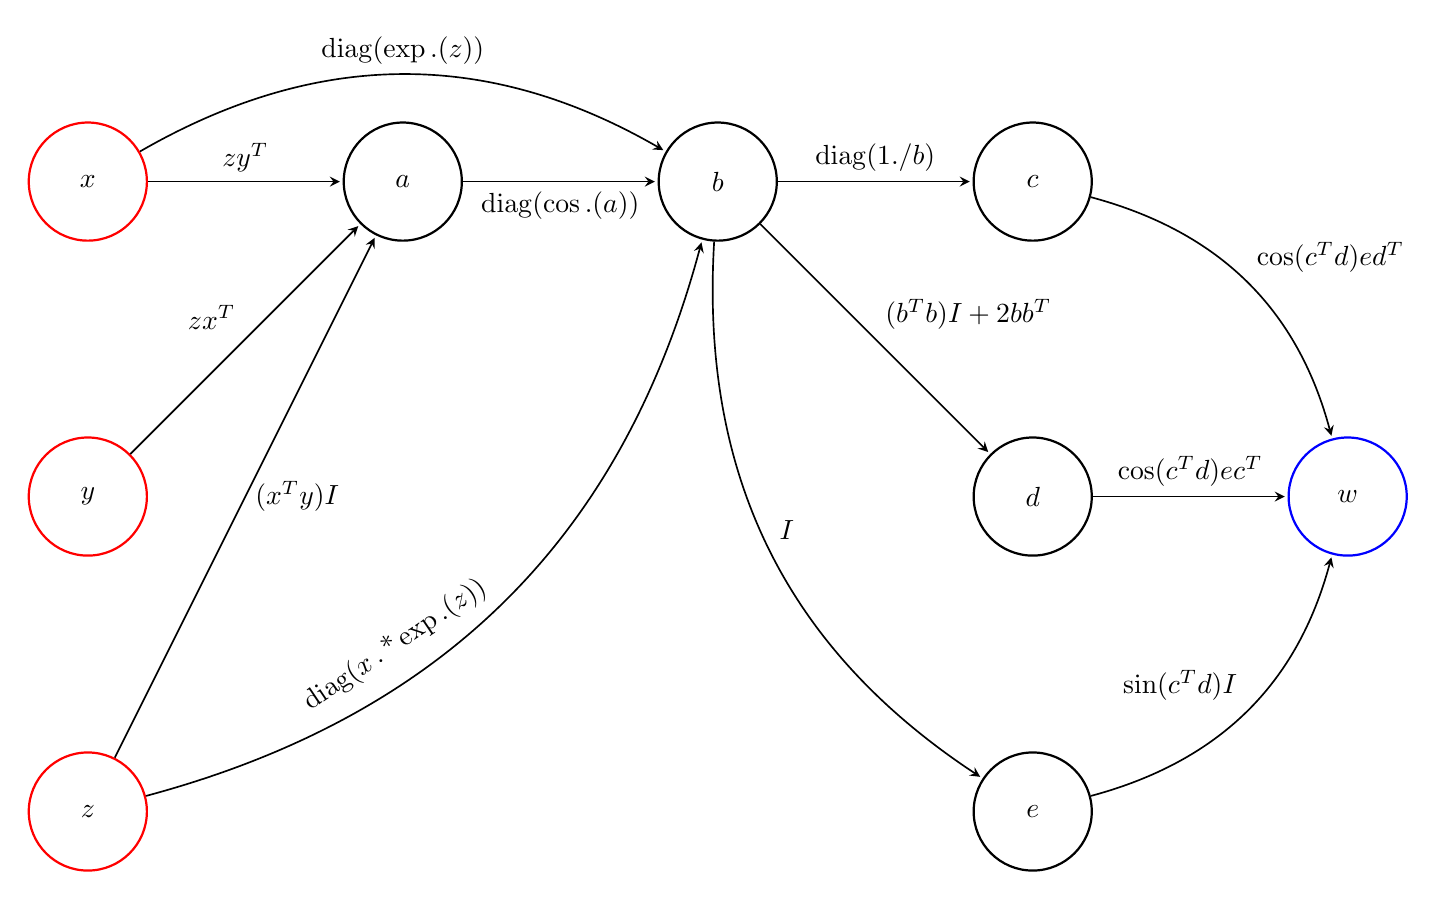
\begin{tikzpicture}[
            > = stealth, % arrow head style
            shorten > = 1pt, % don't touch arrow head to node
            auto,
            node distance = 4cm, % distance between nodes
            semithick, % line style,
        ]

        \tikzstyle{every state}=[
            draw = black,
            thick,
            fill = white,
            minimum size = 15mm
        ]
        \node[state] (a) {$a$};
        \node[state] (x) [left of=a,draw=red] {$x$};
        \node[state] (b) [right of=a] {$b$};
        \node[state] (c) [right of=b] {$c$};
        \node[state] (d) [below of=c] {$d$};
        \node[state] (e) [below of=d] {$e$};
        \node[state] (w) [right of=d,draw=blue] {$w$};
        \node[state] (y) [below of=x,draw=red] {$y$};
        \node[state] (z) [below of=y,draw=red] {$z$};

        \draw[->] (x) edge["$zy^T$"] (a);
        \draw[->] (y) edge["$zx^T$"] (a);
        \draw[->] (z) edge["$(x^T y)I$" right] (a);
        \draw[->] (a) edge["$\diag(\cos.(a))$" below] (b);
        \draw[->] (x) edge[bend left,"$\diag(\exp.(z))$"] (b);
        \draw[->] (z) edge[bend right,"$\diag(x \dotstar \exp.(z))$" rotate=34] (b);
        \draw[->] (b) edge["$\diag(1./b)$"] (c);
        \draw[->] (b) edge["$(b^T b)I + 2bb^T$"] (d);
        \draw[->] (b) edge[bend right,"$I$"] (e);
        \draw[->] (c) edge[bend left,"$\cos(c^T d)e d^T$"] (w);
        \draw[->] (d) edge["$\cos(c^T d) e c^T$"] (w);
        \draw[->] (e) edge[bend right,"$\sin(c^T d) I$"] (w);
    \end{tikzpicture}
\caption{The computational graph for problem 5, with nodes labeled by variables (inputs $x,y,z$ at left, output $w$ at right) and edges labeled by partial derivatives. \label{fig:p5graph}}
\end{center}
\end{figure}
The computational graph is shown in Fig.~\ref{fig:p5graph} (where $\diag v$ denotes the diagonal matrix with the entries of $v$ on the diagonal).

In the following, we refer to the edges above by partial derivatives ($\partial b/\partial a$ for the edge from $a$ to $b$, etcetera) as in class.

\begin{enumerate}

\item Forward mode, which proceeds by going from each input to the output, and finally adding the results:
\begin{enumerate}
\item Paths from $x$. First we compute $\frac{d b}{d x} = \frac{\partial b}{\partial x} + \frac{\partial b}{\partial a}\frac{\partial a}{\partial x} = \diag(\exp.(z)) + \diag(\cos.(a)) (zy^T) $ (summed over two paths).  Then we sum over the paths from $b$ to $w$:
\begin{align*}
\frac{d w}{d x} &= \frac{\partial w}{\partial c} \left[ \frac{\partial c}{\partial b} \frac{d b}{d x} \right]    +  \frac{\partial w}{\partial d} \left[ \frac{\partial d}{\partial b}  \frac{d b}{d x} \right]  + \frac{\partial w}{\partial e} \left[ \frac{\partial e}{\partial b}\frac{d b}{d x} \right]    \\
&= (\cos(c^T d) ed^T)\left[\diag(1./b) \frac{d b}{d x} \right]   + (\cos(c^T d) ec^T) \left[((b^Tb)I + 2bb^T) \frac{d b}{d x}\right] + (\sin(c^T d) I) \left[I \frac{d b}{d x}\right] \, .
\end{align*}
Note that all products are performed \emph{right to left} (inputs to outputs).

\item Paths from $y$: Similarly, we go from $y$ to $b$: $\frac{d b}{d y} = \frac{\partial b}{\partial a} \frac{\partial a}{\partial y} = \diag(\cos.(a)) (zx^T)$ and then from $b$ to $w$:
$$
\frac{d w}{d y} = \frac{\partial w}{\partial c} \left[ \frac{\partial c}{\partial b} \frac{d b}{d y} \right]    +  \frac{\partial w}{\partial d} \left[ \frac{\partial d}{\partial b}  \frac{d b}{d y} \right]  + \frac{\partial w}{\partial e} \left[ \frac{\partial e}{\partial b}\frac{d b}{d y} \right] 
$$
which is exactly the same as the expression for $dw/dx$ except that we have $db/dy$ instead of $db/dx$.   If we parenthesized it from left-to-right, we could factor out the common expressions, but forward mode does not do this!

\item Paths from $z$: Similarly, we go from $z$ to $b$: $\frac{d b}{d z} = \frac{\partial b}{\partial a} \frac{\partial a}{\partial z} + \frac{\partial b}{\partial z}  = \diag(\cos.(a)) ((x^T y)I) + \diag(x \dotstar \exp.(z))$ (two paths) and then again from $b$ to $w$:
$$
\frac{d w}{d y} = \frac{\partial w}{\partial c} \left[ \frac{\partial c}{\partial b} \frac{d b}{d z} \right]    +  \frac{\partial w}{\partial d} \left[ \frac{\partial d}{\partial b}  \frac{d b}{d z} \right]  + \frac{\partial w}{\partial e} \left[ \frac{\partial e}{\partial b}\frac{d b}{d z} \right] \, 
$$
where again there are a lot of repeated calculations that could be factored out \emph{if} we changed the order.
\end{enumerate}

\item Reverse mode: we follow a similar procedure, except this time work from outputs to inputs:

\begin{enumerate}
    \item From $w$ to $b$ (summed over three paths):
    $$
    \frac{dw}{db} = \frac{\partial w}{\partial c} \frac{\partial c}{\partial b} + \frac{\partial w}{\partial d} \frac{\partial d}{\partial b} + \frac{\partial e}{\partial b} \, .
    $$
    Note that this corresponds to factoring out $db/dx$, $db/dy$, and $db/dz$ from the forward-mode expressions above and performing the common multiplications/additions \emph{once}.  Reverse mode does this for you!

    \item From $b$ to $a$: $$\frac{dw}{da} = \frac{d w}{d b} \frac{\partial b}{\partial a} \, .$$ Note that we multiply \emph{on the right} (or equivalently we could transpose everything and multiply on the left).

    \item To $x$ (two paths from $a$ and $b$):
    $$
    \frac{dw}{dx} = \frac{dw}{da} \frac{\partial a}{\partial x} + \frac{dw}{db} \frac{\partial b}{\partial x} =  \left( \frac{d w}{d b} \frac{\partial b}{\partial a} \right) \frac{\partial a}{\partial x} + \frac{dw}{db} \frac{\partial b}{\partial x}
    $$
    
    \item To $y$ (one path from $a$):
    $$
    \frac{dw}{dx} = \frac{dw}{da} \frac{\partial a}{\partial y} = \left( \frac{d w}{d b} \frac{\partial b}{\partial a} \right) \frac{\partial a}{\partial y}
    $$
    
    \item To $z$ (two paths from $a$ and $b$):
    $$
    \frac{dw}{dz} = \frac{dw}{da} \frac{\partial a}{\partial z} + \frac{dw}{db} \frac{\partial b}{\partial z} = \left( \frac{d w}{d b} \frac{\partial b}{\partial a} \right) \frac{\partial a}{\partial z} + \frac{dw}{db} \frac{\partial b}{\partial z}
    $$
    Notice that going from outputs-to-inputs (multiplying left-to-right), as is the style in reverse mode, automatically factored out the common sub-expression $dw/da$ and computes it only once.
\end{enumerate}

\end{enumerate}

\subsection*{Problem 6 (6+6+4 points)}
\begin{enumerate}
\item Suppose that $f(A)$ is a function that maps (real) $m\times m$ matrices
to $m\times m$ matrices, and its derivative is the linear operator
$f'(A)[dA]$. For the Frobenius inner product $\langle X,Y\rangle=\tr(X^{T}Y)$,
it turns out that we typically have 
\[
\left\langle X,f'(A)[Y]\right\rangle =\left\langle f'(A^{T})[X],Y\right\rangle ,
\]
which conceptually corresponds to “transposing” the linear operator
$f'(A)^{T}=f'(A^{T})$. Your job is to show this.
\begin{enumerate}
\item Show this for $f(A)=A^{n}$ for any $n\ge0$. (Hint: From the product
rule, it is easy to see that $f'(A)[dA]=\sum_{k=0}^{n-1}A^{k}dA\,A^{n-1-k}$;
we've already seen this explicitly for several $n$. Combine this
with the cyclic rule for the trace.)\\
\\
It immediately follows that this identity also works for any $f(A)$
described by a Taylor series in~$A$ (any ``analytic'' $f$), such
as $e^{A}$.
\item Show this for $f(A)=A^{-1}$.\\
\\
(You can then compose the above cases to show that it works for any
$f(A)=p(A)q(A)^{-1}$ for any polynomials~$p$ and~$q$, i.e.~for
any rational function of $A$. You need not do this, however.)
\end{enumerate}
\item Consider the function $f(A)=\det(A+\exp(A))$.
\begin{enumerate}
\item Write $f'(A)[dA]$ in terms of $\exp'(A)[dA]$. (You learned how to
compute $\exp'$ in pset~1.)
\item Using the identity from the previous part, write $\nabla f$ in a
way that can be evaluated efficiently (“reverse mode”) using
only one or two evaluations of $\exp$ (and/or $\exp'$) and $\det$,
independent of the size of $A$.
\end{enumerate}
\item Check your answer from the previous part in Julia (or Python etc.):
choose a random $5\times5$ \texttt{A=randn(5,5)} and a random small
\texttt{dA=randn(5,5){*}1e-8}, compute $df=f(A+dA)-f(A)$ and $\nabla f$
(at $A$), and verify that $df\approx\langle\nabla f,dA\rangle$.
Compute $\exp'(A)[dA]$ using the same technique as in pset~1.
\end{enumerate}

\subsubsection*{Solution:}

\begin{enumerate}
    \item 
   \begin{enumerate}
    \item For $f(A) = A^n$, we will use the suggested form of $f'(A)[dA]$ (which is simply the product rule, summing over which of the $n$ $A$ terms becomes $dA$).  Plugging this into the inner product (and using linearity), we find:
    \begin{align*}
    \langle X, f'(A)[Y] \rangle &=
    \sum_{k=0}^{n-1} \tr \left( X^T A^k Y A^{n-1-k} \right) && \text{linearity}\\
    &= \sum_{k=0}^{n-1} \tr \left( A^{n-1-k} X^T A^k Y  \right)
     && \text{cyclic trace}\\
    &=  \tr \left(   \left[ \sum_{k=0}^{n-1} (A^T)^k X (A^T)^{n-1-k} \right] ^T  Y  \right)
     && \text{transpose + linearity} \\
     &= \langle f'(A^T)[X], Y \rangle && \text{Q.E.D.}
    \end{align*}

    \item For $f(A) = A^{-1}$, the proof is similar, relying on the fact that $(A^{-1})^T = (A^T)^{-1}$:
    \begin{align*}
    \langle X, f'(A)[Y] \rangle &= -\tr\left( X^T A^{-1} Y A^{-1} \right) && \text{derivative of }A^{-1}\\
    &= -\tr\left( A^{-1} X^T A^{-1} Y  \right) && \text{cyclic trace}\\
    &= \tr\left( [-(A^T)^{-1} X (A^T)^{-1}]^T Y  \right) && \text{transpose}\\
     &= \langle f'(A^T)[X], Y \rangle && \text{Q.E.D.}
    \end{align*}
    
    \end{enumerate}
    
    \item Here, $f(A)=\det(A+\exp(A))$.
     
   \begin{enumerate}
   \item
   From class, we saw that $\det'(X)[dX] = \det(X) \tr(X^{-1} dX)$.  Here, $X = A + \exp(A)$, so by the chain rule we can plug in $dX = dA + \exp'(A)[dA]$:
    $$
    df = f'(A)[dA] = \boxed{\det(\underbrace{A + \exp(A)}_X) \tr\left( X^{-1} (\underbrace{dA +\exp'(A)[dA]}_{dX})  \right)} \, .
    $$

    \item We need to write $df = \langle \nabla f, dA \rangle = \tr[(\nabla f)^T dA ]$.  From above, already have one term in this form, giving us a term $\det(X)X^{-T}$ in the gradient.  The other term is our $\exp'(A)$ term, and we can use the theorem in the previous part to shift this to act on $X$ by transposing $A$. (Making $\exp'$ act ``to the left'' or ``transposing the operator'' is, in fact, an instance of reverse-mode or ``adjoint'' differentiation.)  Hence, we have:
    $$
    df = \det(X) \langle X^{-T} + \exp'(A^T)[X^{-T}], dA \rangle
    $$
    which gives
    $$
    \boxed{ \nabla f = \underbrace{\det(X)}_{f(A)} \left( X^{-T} + \exp'(A^T)[X^{-T}] \right) } \, .
    $$
    where $X = A + e^A$ and $X^{-T} = (X^{-1})^T = (X^T)^{-1}$.  This only requires us to compute one determinant (which can be re-used from the computation of $f(A)$), one $\exp$, one $\exp'$ application, and one inverse $X^{-T}$.\footnote{Note that matrix inversion is \emph{much} faster than matrix exponentiation, although both operations have $O(m^3)$ cost for $m \times m$ matrices---about $10\times$ faster on my 2021 laptop for $m=1000$.  Also, both matrix inversion and determinants start with LU factorization, so they can share some computation.}
    
    \end{enumerate}
    
    \item See accompanying Julia notebook for finite-difference check.
\end{enumerate}

\end{document}
